% Made up for the tikra benchmark.
% A rose (coxcomb) chart in the style of Florence Nightingale's 1858 diagram: twelve months,
% each wedge's area its count (made-up numbers), stacked by cause.
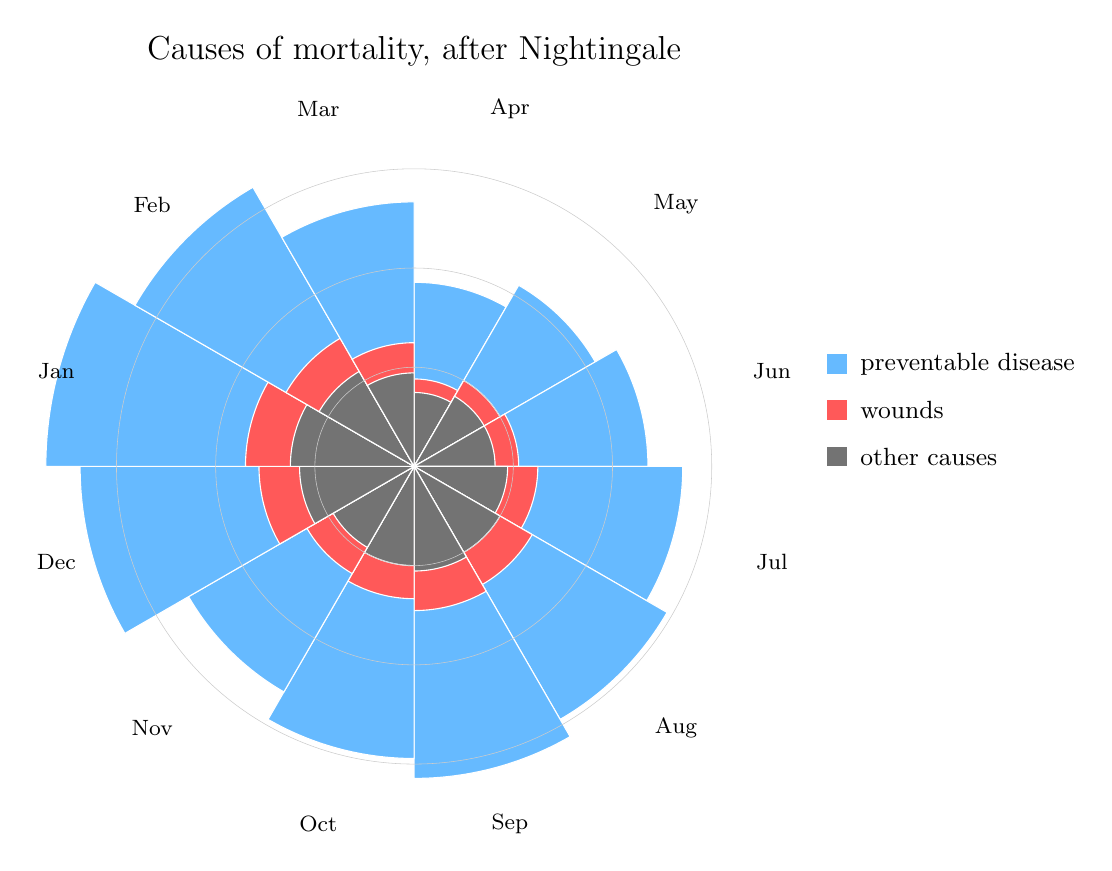
\begin{tikzpicture}[scale=0.42]
  \foreach \month/\disease/\wounds/\other [count=\i from 0] in
      {Apr/24/2/5, May/31/3/6, Jun/40/4/6, Jul/52/6/8, Aug/61/8/9, Sep/70/9/10, Oct/62/7/9,
       Nov/48/6/8, Dec/80/10/12, Jan/98/12/14, Feb/75/9/11, Mar/50/6/8} {
    \pgfmathsetmacro\s{90 - 30*\i}
    \pgfmathsetmacro\e{\s - 30}
    \pgfmathsetmacro\rd{sqrt(\disease + \wounds + \other)}
    \pgfmathsetmacro\rw{sqrt(\wounds + \other)}
    \pgfmathsetmacro\ro{sqrt(\other)}
    \fill[blue!45!cyan!60, draw=white, thin] (0,0) -- (\s:\rd) arc (\s:\e:\rd) -- cycle;
    \fill[red!65, draw=white, thin] (0,0) -- (\s:\rw) arc (\s:\e:\rw) -- cycle;
    \fill[black!55, draw=white, thin] (0,0) -- (\s:\ro) arc (\s:\e:\ro) -- cycle;
    \pgfmathsetmacro\m{\s - 15}
    \node[font=\footnotesize] at (\m:11.2) {\month};
  }
  \foreach \r in {3,6,9} \draw[gray!40, very thin] (0,0) circle (\r);
  \fill[blue!45!cyan!60] (12.5,2.8) rectangle (13.1,3.4);
  \node[anchor=west, font=\small] at (13.2,3.1) {preventable disease};
  \fill[red!65] (12.5,1.4) rectangle (13.1,2.0);
  \node[anchor=west, font=\small] at (13.2,1.7) {wounds};
  \fill[black!55] (12.5,0) rectangle (13.1,0.6);
  \node[anchor=west, font=\small] at (13.2,0.3) {other causes};
  \node[font=\large, anchor=south] at (0,11.8) {Causes of mortality, after Nightingale};
\end{tikzpicture}
